\chapter{Method}\label{chap:method}

The method used will try to achieve the project objectives with correct results, and avoid or lower risks for project failure.


The project is a failure if the results are invalid, or cannot be realized into a real solution, or are so low quality that the project does not receive further development.
The project is also a failure if it does not provide any value for its stakeholders.


The following sections describe the key elements to the method.
There is an overarching approach, called Design Science Research.
It has 6 phases, from problem identification, to development, to evaluation and communication.
There is no methodology given by Design Science Research for executing the development phase.
Therefore, a method for this phase must be crafted from experience and existing practice.
The development phase consists of requirements engineering methods, and software development methods.

% Design Science, build and evaluate.
\section{Design Science Research}

Design Science Research in information systems is a methodology for creating new knowledge by designing, building and evaluating software \glspl{artifact}.
It may not be as widely known as ``the scientific method'' is, and is therefore explained in more detail.

\paragraph{Design}
\textit{Design} in information systems is an iterative process and a resulting software artifact. A software artifact is to be built to solve problems for humans, and evaluated to prove it solves the problems~\cite[p.~2]{alanhevnerDesignResearchInformation2010}.


\paragraph{Research}
\textit{Research} is an activity that adds new knowledge and understanding about something.
Research should be systematical and use data to answer questions, solve problems and provide understanding~\cite[p.~2,3]{alanhevnerDesignResearchInformation2010}.

\paragraph{Design Science Research}
\textit{Design Science Research} is an approach to research where knowledge is created by design.
It is defined by \textcite[p.~5]{alanhevnerDesignResearchInformation2010} as follows:

\begin{quote}
  \textit{``Design science research is a research paradigm in which a designer answers questions relevant to human problems via the creation of innovative artifacts, thereby contributing new knowledge to the body of scientific evidence.
  The designed artifacts are both useful and fundamental in understanding that problem.''}
\end{quote}

The end goal of a Design Science Research project is to create information technology \glspl{artifact}, that improve exiting solutions or solve a problem for the first time~\cite[p.~6]{alanhevnerDesignResearchInformation2010}.
A similar methodology may also be known under the name \textit{Design and Creation}, as presented by \textcite[p.~108]{oatesResearchingInformationSystems2006}.
According to \textcite{alanhevnerDesignResearchInformation2010}, the artifacts are generally classified as \textit{constructs}, \textit{models}, \textit{methods}, \textit{instantiations} or \textit{better design theories}%
\footnote{This thesis aims to produce an instantiation: an implemented or prototype system. The thesis also seeks to advance on \textit{better design theories}, with regards to software architecture and protocol design.}.
A very important aspect of Design Science Research is \textit{evaluation} of the artifact.
The evaluation is the process that uncovers new knowledge, and separates the process from routine design~\cite[p.~7]{alanhevnerDesignResearchInformation2010}.
There are many aspects that could be evaluated, but the aspects that \textit{should} be evaluated are those that are related to the reason for creating the artifact in the first place; the aspects related to the research objectives~\cite[p.~115]{oatesResearchingInformationSystems2006}.


\subsection{Methodology}

% TODO

\begin{figure}[htbp]  % order of priority: h here, t top, b bottom, p page
  \centering
  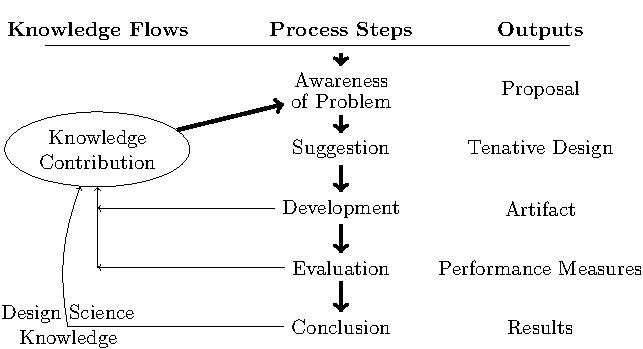
\includegraphics[width=\textwidth]{figures/dsrm-flow.pdf}
  \caption[Design Science Research Process Model]{\textbf{Design Science Research Process Model}. The general process followed by Design Science Research. The figure is recreated based on Figure 3 in \textcite[p.~11]{vijayvaishnaviDesignScienceResearch2019}}\label{fig:dsrpm}
\end{figure}

* Design Science. Build and evaluate value. Contribute to knowledge base. Is this software we need?

\subsection{Evaluation}

* How the different tests were created.

\section{Requirements Engineering}

\subsection{Requirements Extraction}

* Requirements engineering by extraction. Skip user testing for requirement validation. Use cases and existing product.

\subsection{Source Code Analysis of Similar Projects}
* Source code inspection of similar projects. Use the same architecture, design patterns, build systems, software dependencies. Ensures familiarity for the ecosystem, and uses already empirically validated designs.

\subsection{Stakeholder Discussion}

* Talks with supervisor. Discovers use cases, features and other wants.

\subsection{Use Cases and Prototyping}

* Creating a prototype or early version and trying to use it will reveal missing requirements. (For example here: copy-paste, keyboard shortcuts etc)

\section{Development Methodologies}

\subsection{Agile}

* Agile planning. Avoid big upfront design and specification. Change plans as new discoveries become evident.

\subsection{Iterative Development}
* Iterative development. Work on one component at the time, up to a minimum level of functionality. Then come back later and add more.


\subsection{Lean and Minimum Viable Product}

* Lean development. Create a minimum viable product and see if it works.

\subsection{Domain Driven Design}

* Domain driven design. Increase software quality, developer understanding and software re-use with layered architecture, domain layer and ubiquitous domain language.

\subsection{Test Driven Development}

* Test driven development, where applicable. Verify behavior of critical logic, to reduce bugs and increase developer confidence and speed.

\subsection{Tracer Bullets}
* Tracer bullets. Reduce risk from integration by connecting all the major components, before developing any component fully.

\subsection{Prototyping}

* Pre-project with prototyping. Reduce risk by testing feasibility early. Creates more learning, validates requirements and discovers new requirements.
